% Arrhenius plot with film-diffusion, pore-diffusion and kinetic regimes.
% ln k_eff is a smooth minimum of three straight lines with slopes 0.3 : 2 : 4
% (film : E_a/2 : E_a), crossing at 1/T = 0.35 and 0.70 (arbitrary units).
\documentclass[border=4pt]{standalone}
% Shared style for the ch. 10 schematic plots (figures/src/*.tex).
% Build one figure:  lualatex <name>.tex   then see README.md for the PNG step.
\usepackage{amsmath}
\usepackage{pgfplots}
\pgfplotsset{compat=1.18}
\usetikzlibrary{arrows.meta}

\definecolor{matblue}{HTML}{0072BD}
\definecolor{matorange}{HTML}{D95319}

\pgfplotsset{
  schematic/.style={
    width=8cm, height=6.2cm,
    axis lines=left,
    axis line style={-{Stealth[length=2.5mm]}, line width=0.8pt},
    xtick=\empty, ytick=\empty,
    xmin=0, ymin=0,
    clip=false,
    every axis x label/.style={at={(current axis.right of origin)}, anchor=north east, yshift=-4pt},
    every axis y label/.style={at={(current axis.above origin)}, anchor=north east, xshift=-4pt},
    label style={font=\normalsize},
    samples=200,
  },
  curve/.style={line width=1.4pt, color=matblue},
  guide/.style={line width=0.8pt, dashed, color=black!60},
}

\begin{document}
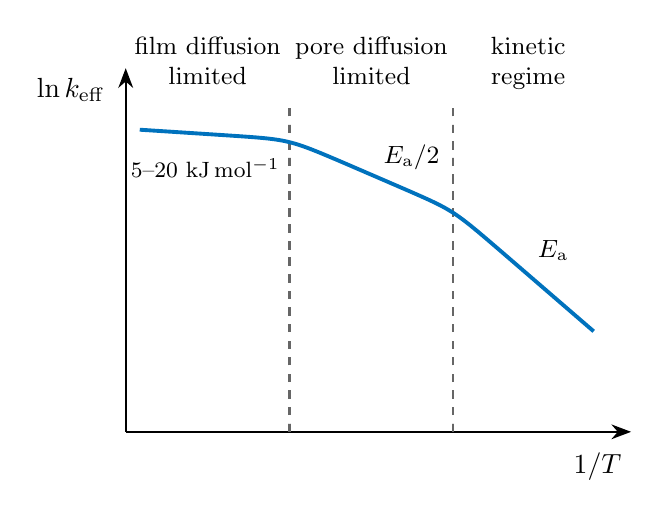
\begin{tikzpicture}
\begin{axis}[schematic, xmax=1.08, ymin=0, ymax=3.6,
    xlabel={$1/T$}, ylabel={$\ln k_\mathrm{eff}$},
    declare function={
      lf(\x) = 3.0 - 0.3*\x;
      lp(\x) = 3.595 - 2*\x;
      lk(\x) = 4.995 - 4*\x;
      s = 0.04;
      keff(\x) = -s*ln(exp(-lf(\x)/s) + exp(-lp(\x)/s) + exp(-lk(\x)/s));
    }]
  \addplot[guide, domain=0:3.25] (0.35, {x});
  \addplot[guide, domain=0:3.25] (0.70, {x});
  \addplot[curve, domain=0.03:1] {keff(x)};
  \node[font=\small, align=center, anchor=south] at (axis cs:0.175,3.25) {film diffusion\\limited\strut};
  \node[font=\small, align=center, anchor=south] at (axis cs:0.525,3.25) {pore diffusion\\limited\strut};
  \node[font=\small, align=center, anchor=south] at (axis cs:0.86,3.25) {kinetic\\regime\strut};
  \node[font=\footnotesize, anchor=north] at (axis cs:0.17,2.8) {$5$--$20\ \mathrm{kJ\,mol^{-1}}$};
  \node[font=\small, anchor=south west] at (axis cs:0.53,2.5) {$E_\mathrm{a}/2$};
  \node[font=\small, anchor=south west] at (axis cs:0.86,1.6) {$E_\mathrm{a}$};
\end{axis}
\end{tikzpicture}
\end{document}
